
\section*{TP 6 - 7 : Cinématique des fluides parfaits}

\subsection*{Loi de comportement générale des fluides}
\begin{equation}
\tau _{ij} = -p \delta _{ij} +\lambda \delta _{ij} V_ {kk} + 2\mu V_{ij}
\end{equation}
où $\lambda$ et $\mu$ sont les coefficients de viscosité.

\subsection*{Théorème de Bernouilli}
\begin{itemize}
	\item Hypothèses :
		\begin{itemize}
			\item Fluide parfait $\Rightarrow \tau _{ij} = -p \delta _{ij}$
			\item Fluide incompressible $\Rightarrow \rho ^{\bullet} = 0$
			\item Ecoulement permanent $\Rightarrow \partial _0 v_i = 0$
		\end{itemize}
	
	\item Théorème :\\
		Dans un écoulement permanent d'un fluide parfait soumis à un champ de force massique dérivant d'un potentiel, l'énergie spécifique totale est constante le long d'une ligne de courant.
		\begin{equation}
			\epsilon = gz + \frac{p}{\rho} + \frac{v^2}{2} = cst
		\end{equation}
		le long d'une ligne de courant.\\
		\textbf{Attention :} $\epsilon$ est une énergie par unité de masse $[J/kg] = [m^2/s^2]$
		
		\item Charge :
			\begin{equation}
				H = \frac{\epsilon}{g} = z + \frac{p}{\rho g} + \frac{v^2}{2 g}
			\end{equation}
\end{itemize}

\subsection*{Conservation du débit}
Permet de calculer la vitesse du fluide si la surface de passage change 
\begin{equation}
	Q = vS = cst
\end{equation}

\subsection*{Cavitation}
\begin{itemize}
	\item Correspond au changement de phase dans un fluide
	\item Si $p \searrow \, \Rightarrow T \nearrow$, formation de bulles dû à la faible pression et il y a formation de bulles. Il y a donc cavitation lorque $p < p_{vap}$ (tension de vapeur)
	\item Ecoulement impossible
\end{itemize}

\subsection*{Remarque}
\begin{itemize}
	\item Si le réservoir est grand on considère que l'écoulement est assez lent que pour faire varier la hauteur
	\item Le \textit{principe de Pascal} ne s'applique qu'en statique ! En dynamique on utilise \textit{Bernouilli}
\end{itemize}

\subsection*{Ligne de charge, piézométrique et de courant}
\begin{itemize}
\item La première est juste la représentation de H en fonction de l'endroit (cst)
\item La deuxième consiste à reporter $v^2/(2 g)$ selon l'endroit \textbf{mais par rapport à la charge !}
\item La dernière est la représentation de la hauteur de la ligne d'écoulement en fonction de l'endroit. \textbf{La différence avec la courbe piézométrique donne $p/\rho g$}.
\end{itemize}
\begin{center}
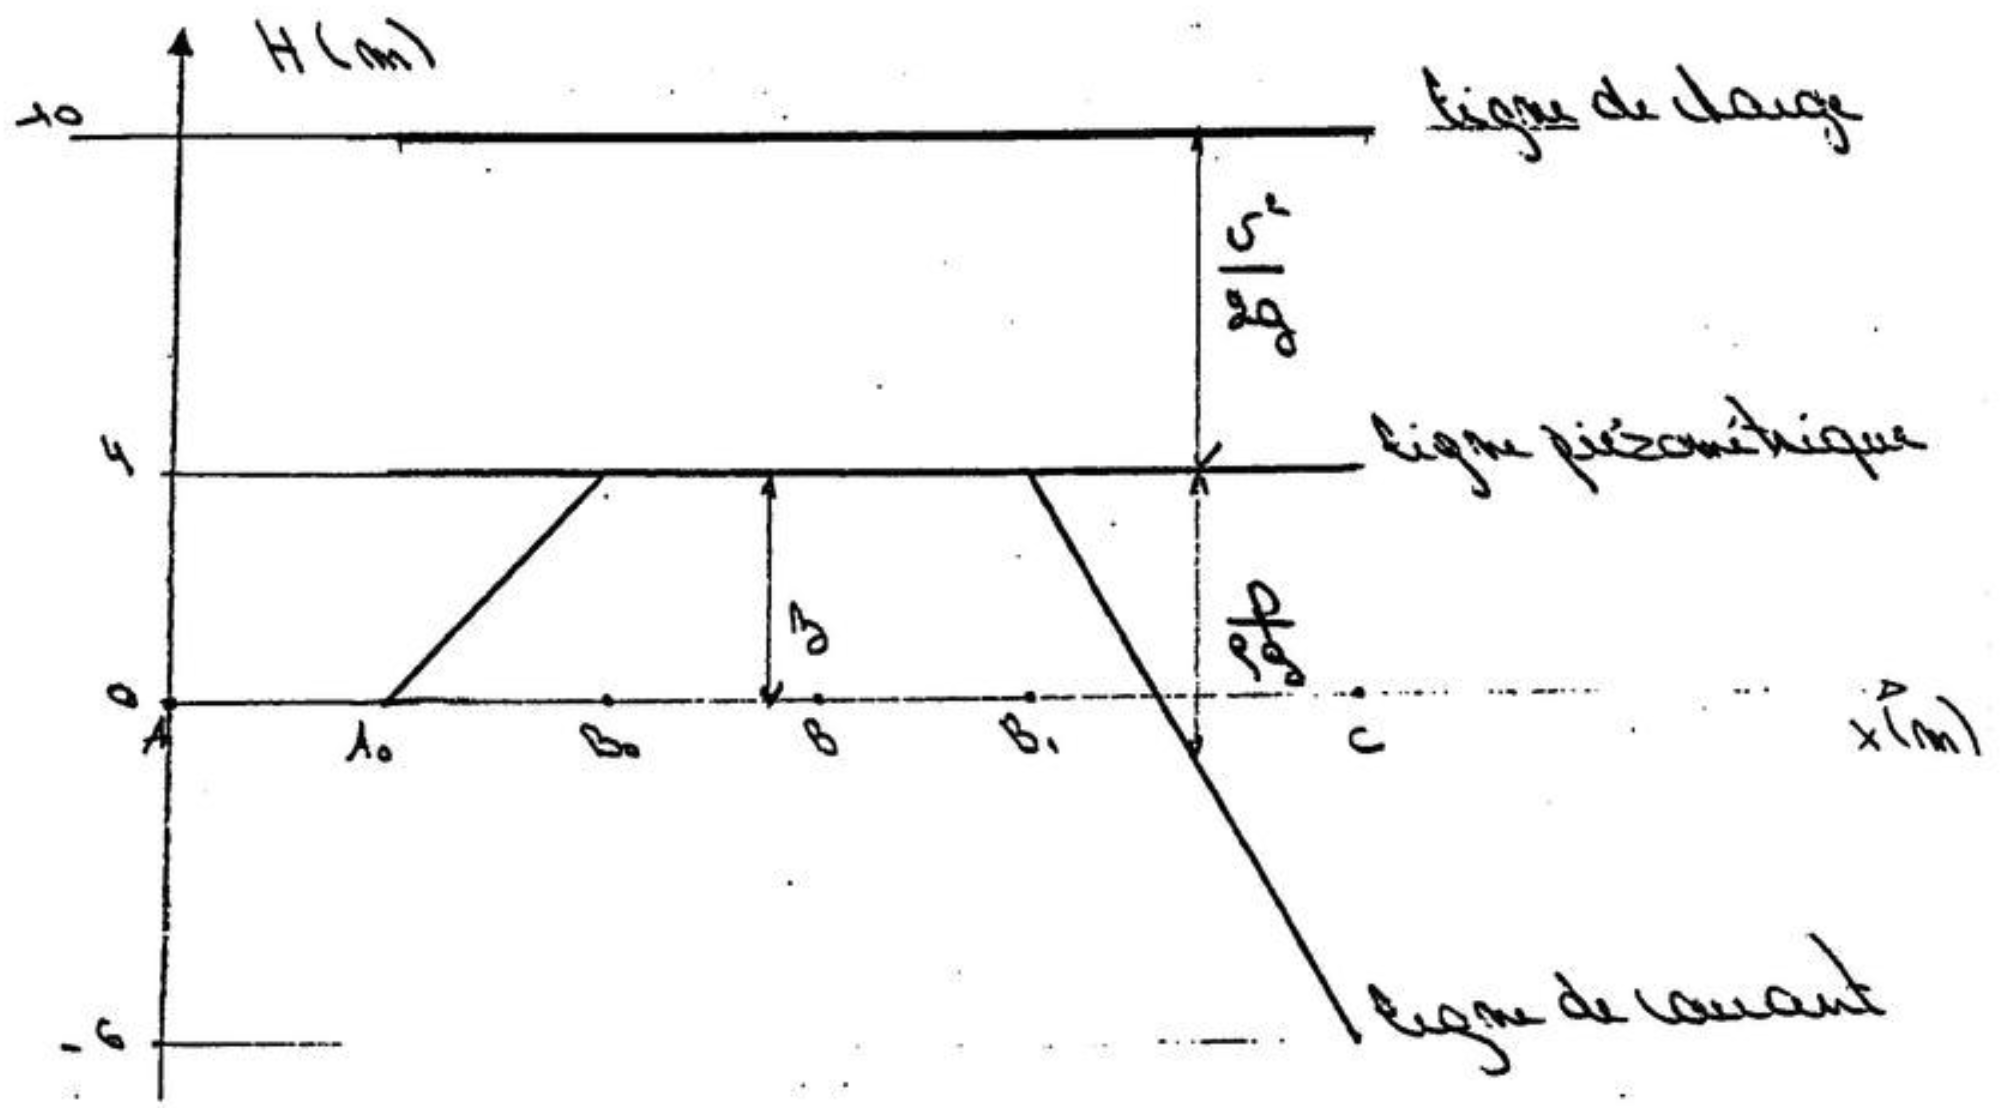
\includegraphics[scale=0.3]{tp6}
\end{center}